

Este algoritmo tiene complejidad $O(m \log m)$. Sin embargo, como vimos anteriormente, esta no es una cota ajustada, si no que nuestro algoritmo puede acotarse más ajustadamente por $O(m \log n)$.

De todos modos, primero confirmemos que nuestro algoritmo tiene complejidad $O(m \log m)$.

\begin{figure}[H]
 \centering
	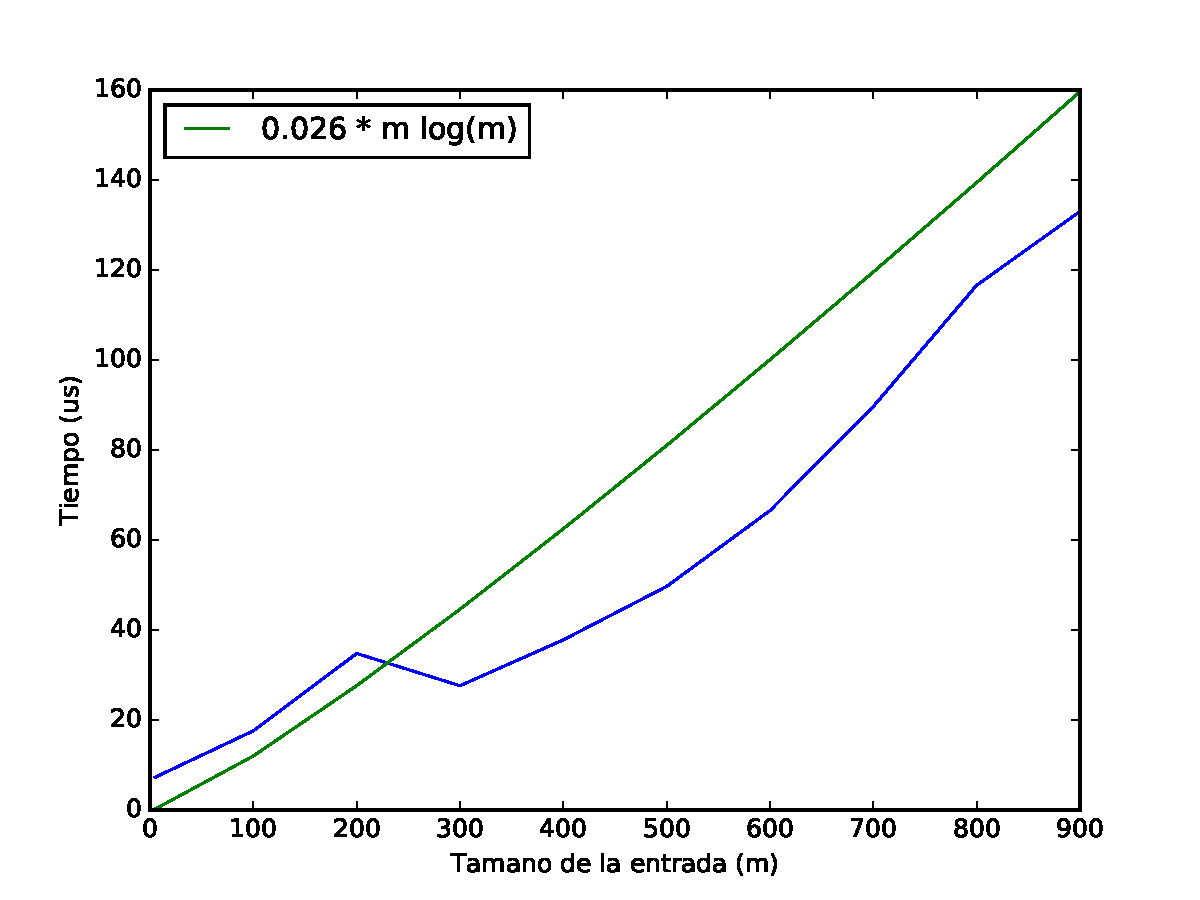
\includegraphics[width=0.9\textwidth]{img/exp/problema2-promedio.pdf}
	\caption{\footnotesize Tiempo que toma el algoritmo en $\mu$s para una entrada de tamaño $m$. $n$ al azar.}
	\label{fig:problema2-promedio}
\end{figure}

Sin embargo, como dijimos antes, esta cota no es ajustada. Esto puede verse en el siguiente gráfico. Lo que hicimos fue tomar $m$ fijo como antes, pero no mostrar las mediciones condensadas en un punto, si no que ahora mostramos todas las mediciones tomadas para un mismo $m$, variando $n$. 

Como puede verse, la varianza es altísima.

\begin{figure}[H]
 \centering
	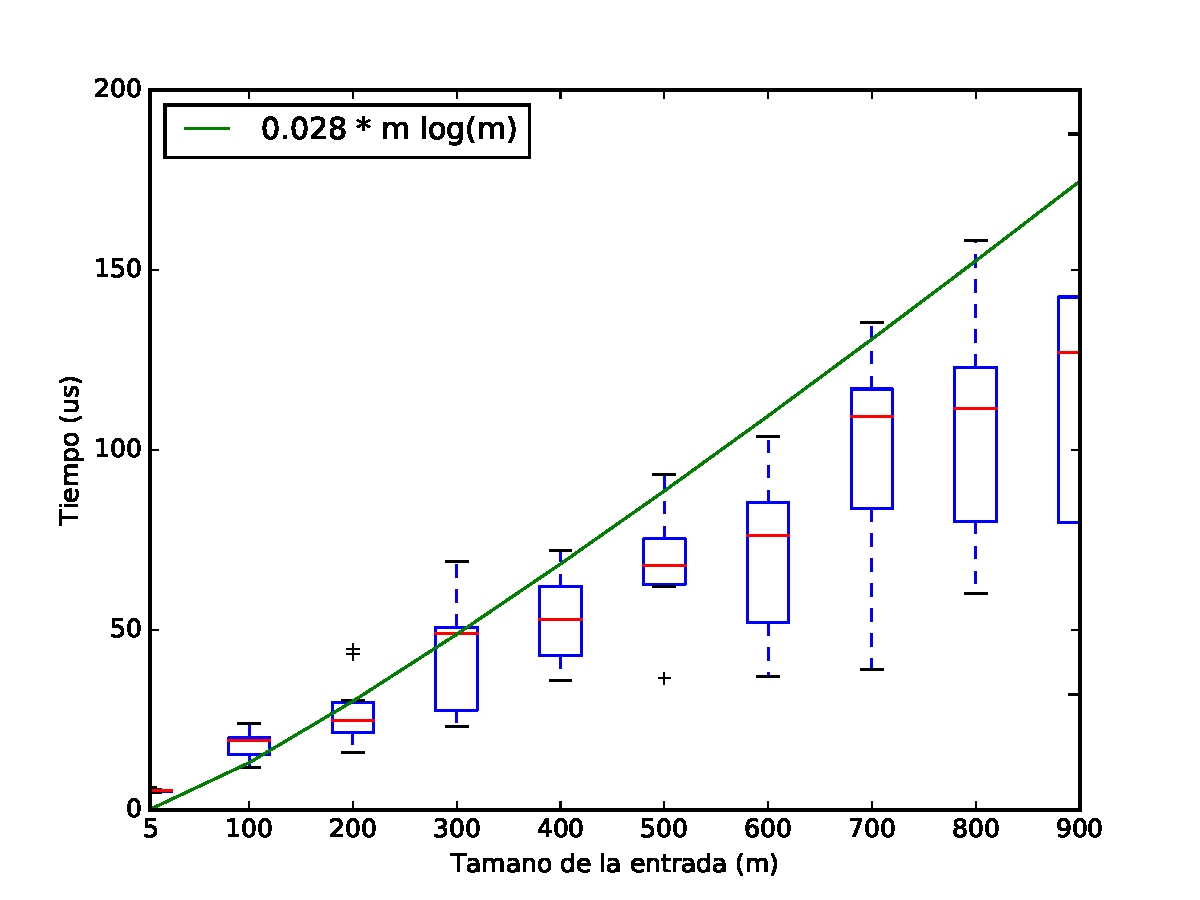
\includegraphics[width=0.9\textwidth]{img/exp/problema2-promedio2.pdf}
  \caption{\footnotesize Tiempo que toma el algoritmo en $\mu$s para una entrada de tamaño $m$. $n$ al azar. Se indican los valores del primer al tercer cuartil con un rectángulo azul y la mediana con una linea roja. El máximo y minimo se indican con lineas negras arriba y abajo del rectángulo.}
	\label{fig:problema2-promedio2}
\end{figure}

Esto se debe a que en realidad, la complejidad no es independiente de $n$, si no que para $m$ fijo, si se toma un $n$ más pequeño, el tiempo que tarde el programa va a ser mucho menor que con un $n$ un poco más grande.

Como dijimos antes, una cota más ajustada para nuestro algoritmo es la de $O(m \log n)$, así que pasemos a confirmar esto experimentalmente.

\begin{figure}[H]
 \centering
	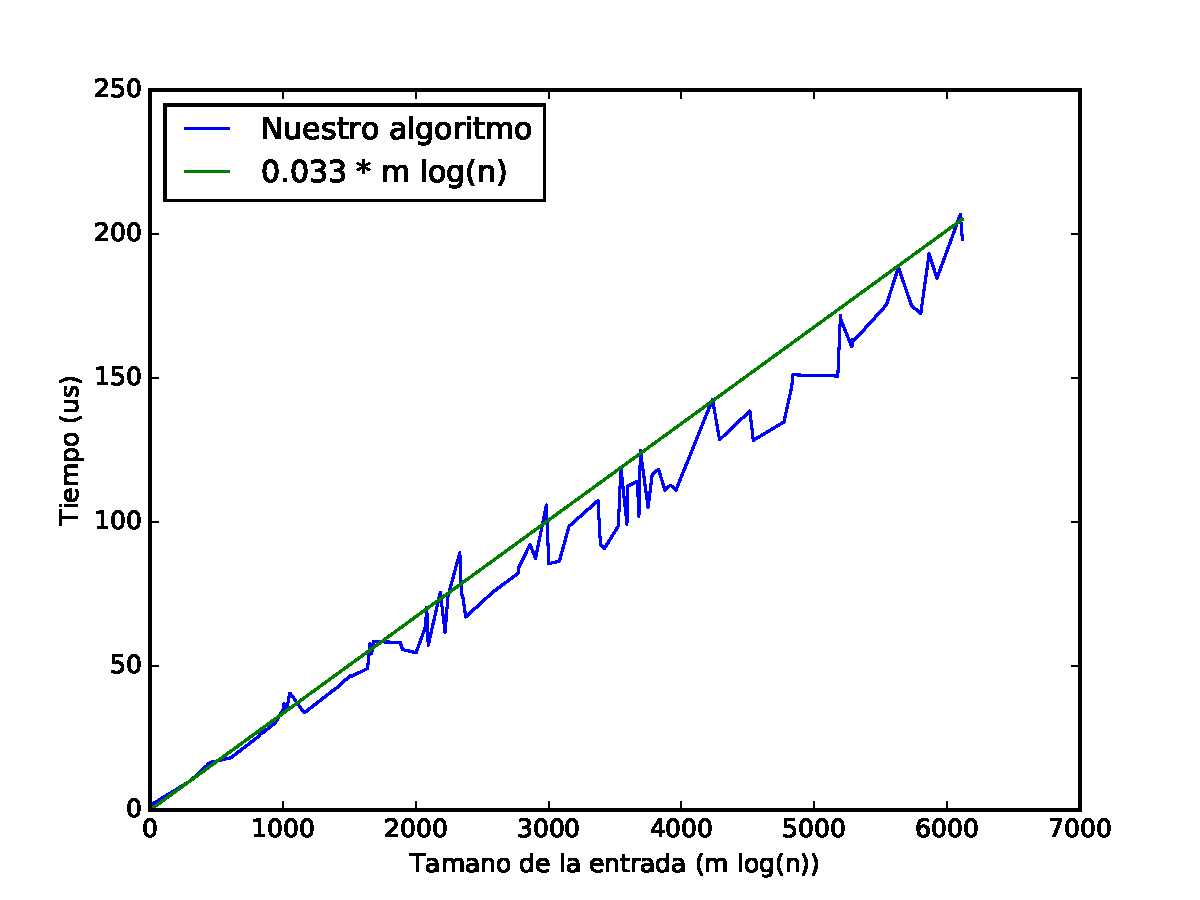
\includegraphics[width=0.9\textwidth]{img/exp/problema2-posta.pdf}
	\caption{\footnotesize Tiempo que toma el algoritmo en $\mu$s para una entrada de tamaño $m \log n$.}
	\label{fig:problema2-posta}
\end{figure}


\subsubsection{M\'etodo de experimentación}

Para generar los grafos al azar, al igual que en el problema anterior, usamos el algoritmo descripto en el apéndice.

Para las figuras \ref{fig:problema2-promedio} y \ref{fig:problema2-posta} tomamos 100 mediciones (en el caso de \ref{fig:problema2-promedio} tomamos algunas más, porque para cada $m$ tomabamos varios $n$ distintos, al rededor de 10, o sea que las mediciones en este caso eran de 1000, 100 por cada $n$). De todas estas mediciones tomamos la mediana, que es lo que se representó en el gráfico.

